\documentclass[11pt]{article}

\usepackage[margin=1in]{geometry}
\usepackage{amsmath}
\usepackage{fontspec}
\usepackage{unicode-math}
\usepackage{microtype}
\usepackage{parskip}
\usepackage{booktabs}
\usepackage{array}
\usepackage{graphicx}
\usepackage{placeins}

\setlength{\emergencystretch}{3em}

% Unicode math symbols in running text (shared with the MultiBench build).
% Map math symbols that the text font lacks to math-mode equivalents.
% (Adapted unchanged from the JaleesBench paper's preamble.tex.)
\usepackage{newunicodechar}
\newunicodechar{→}{\ensuremath{\rightarrow}}
\newunicodechar{←}{\ensuremath{\leftarrow}}
\newunicodechar{≤}{\ensuremath{\leq}}
\newunicodechar{≥}{\ensuremath{\geq}}
\newunicodechar{≈}{\ensuremath{\approx}}
\newunicodechar{−}{\ensuremath{-}}
\newunicodechar{×}{\ensuremath{\times}}
\newunicodechar{≠}{\ensuremath{\neq}}
\newunicodechar{·}{\ensuremath{\cdot}}


\providecommand{\tightlist}{%
  \setlength{\itemsep}{0pt}\setlength{\parskip}{0pt}}

\usepackage{natbib}
\setlength{\bibsep}{2pt plus 0.3ex}

\usepackage{xcolor}
\definecolor{citecol}{HTML}{1A4D8F}
\usepackage[colorlinks=true,citecolor=citecol,linkcolor=citecol,urlcolor=citecol]{hyperref}
\usepackage[nameinlink]{cleveref}
\crefname{section}{section}{sections}
\Crefname{section}{Section}{Sections}
\crefname{table}{Table}{Tables}
\Crefname{table}{Table}{Tables}

% DRAFT SKELETON (2026-08-05): the experiment is mid-flight. Sections whose
% data has not landed carry \todo markers — SFT eval sweep (capability,
% MultiBench-descriptive), the DPO stage, and final numbers arrive with the
% pre-DPO checkpoint and after. Do not circulate until they are filled.
\newcommand{\todo}[1]{\textcolor{red}{\textbf{[TODO: #1]}}}

% TODO: working title (Waleed's phrasing, 2026-08-05); confirm before submission.
\title{MultiWeights: A Model Without Omissive Bias for
Faiths\thanks{Draft. Author list omitted for now.}}
\author{}
\date{}

\begin{document}

\maketitle

\begin{abstract}
MultiBench measured that frontier models fail undeclared believers mostly
through \emph{recognition}, not capability: told whom they serve, models
largely can serve them --- the failure is omissive. This paper asks whether
that recognition can be \emph{internalized rather than prompted}: we
fine-tune an open-weights model (Gemma-4-31B-it) on its own guided-framing
counsel across MultiBench's seven traditions --- judge-filtered context
distillation, then on-policy DPO --- and measure whether the unstated
behavior rises toward the guided ceiling without leaking faith into secular
contexts. The recipe generalizes the single-tradition JaleesModel result
\citep{jaleesbench2026} to seven traditions at once. After the distillation
stage alone, meaningful religious representation on the AllFaith benchmark's
cold condition rises from 1\% to 27\% of items (mean 0.113 → 1.147),
decisively above the published 0--2\% frontier ceiling
\citep{omissivebias2026}, with \emph{zero} measured leakage into coding,
factual, mathematical, or secular-practical tasks and general capability
essentially preserved (GSM8K $+3.0$, IFEval $-1.1$, MMLU $-2.3$ points).
On MultiBench's own descriptive read, the distilled model's unstated
means flip positive in all seven traditions in aggregate; an
exposure-stratified holdout analysis shows that in-distribution read is
roughly 4$\times$ exposure-concentrated, with a smaller but real
transferable component ($+0.22$ on strictly untrained scenarios) --- the
paper's load-bearing claims therefore rest on the out-of-distribution
instruments. The on-policy preference stage then calibrates the
shape: meaningful representation rises further (27\% $\to$ 30\%) while
the maximal-representation spike tempers and the opted-out over-mention
regression repairs fully to the base rate, with capability still flat ---
achieved despite near-chance preference accuracy in training, because the
distilled policy already samples good counsel in most cells. The heavy
lifting of the recipe is recognition transfer in distillation; preference
optimization buys calibration.
\end{abstract}

\section{Introduction}\label{sec:intro}

MultiBench's central finding is that the field is \emph{unknowing, not
unwilling}: across seven traditions, five frontier subjects, and three
framings, most of the cross-tradition difficulty difference dissolves once
the model is told whom it is serving, and the guided ceilings show the
competence already exists. The engineering response suggested by that
finding is a system prompt. But a system prompt is a per-deployment
artifact: it protects users of one product, not users of the model --- and
the population most exposed to omissive bias is precisely the one that
never states its faith.

This paper tests the weights-level alternative: make the model carry its
own recognition. We apply judge-filtered context distillation --- training
the model on \emph{its own} guided-framing counsel, with the guide removed
from the training view --- followed by on-policy preference optimization,
and ask three questions:

\begin{enumerate}
\tightlist
\item
  Does internalized recognition close the omission? (Measured on the
  AllFaith Religious Representation Benchmark's cold condition
  \citep{omissivebias2026}, where frontier models score 0--2\%.)
\item
  Does it stay put? (Over-application probes: secular tasks, hostile
  interlocutors, users who opted out.)
\item
  What does it cost? (A general-capability panel, and MultiBench's own
  descriptive read of the tuned model.)
\end{enumerate}

The recipe is the JaleesModel procedure from the JaleesBench programme
\citep{jaleesbench2026}, which produced these effects for a single
tradition (Sunni Islam); MultiWeights is the test of whether one model can
carry seven traditions' recognition at once --- the weights-level analogue
of MultiBench's claim that the construct is faith-general.

\section{Method}\label{sec:method}

\subsection{Subject model and prerequisite collection}\label{sec:subject}

The subject is \textbf{Gemma-4-31B-it}. Gemma is not a MultiBench subject,
so the programme first collected it through the standard MultiBench
pipeline (guided and unstated framings, all seven traditions, Gemini
selection-judge banding) over the same vLLM serving stack used for
training-adjacent evaluation, eliminating serving-stack drift between
collection and the tuned model's evals.

\subsection{Stage 0: the samplability gate}\label{sec:samplability}

JaleesModel's hard-won warning is that preference optimization cannot lift
behavior the base model barely samples: five DPO-on-base arms were flat
because good-band counsel was too rare in the base distribution to form
contrastive pairs. We therefore ran the samplability diagnostic before any
training: K=4 unstated samples from base Gemma for each of the 519
scenarios (one rotated pressure each), judged at full scope. The result
mandates the two-stage design: \textbf{55\% of scenarios are never-good
across all four samples} --- and the failure concentrates exactly where the
tune matters most (Sunni Islam 71\%, Roman Catholicism 67\% never-good,
against Buddhism 29\%, Taoism 33\%). The K=4 score distribution is bimodal
(51.9\% of samples at −1.0, 24.3\% at +1.0). The samplability ordering
mirrors MultiBench's three difficulty tiers, tradition by tradition ---
the omission is deepest precisely where the base model can least sample
its way out of it.

\subsection{Stage 1: judge-filtered context distillation}\label{sec:sft}

Training examples are the subject's \emph{own} guided-framing sittings that
the selection judge scored in the good band (≥ +1 at both scopes), screened
(no references to the guide, no dangling citations), and re-rendered
\emph{bare} --- the guide lives outside the judged turns, so the transform
is exact. The pooled seven-tradition set is \textbf{2{,}732 examples}; pool
shares track corpus shares (no per-tradition balancing; Sunni Islam is if
anything under-represented relative to its bank size), and there is no
scenario holdout --- evaluation is on separate instruments, not held-out
scenarios.

Fine-tuning is LoRA (r = 32, $\alpha$ = 32, dropout 0) on the bf16 base ---
244M trainable parameters, 0.78\% --- with masked token-mean NLL on
assistant tokens, lr $5\times10^{-5}$, effective batch 8, 2 epochs (683
steps), on a single NVIDIA B200 (1h48m; loss 2.64 → 0.47). The recipe is
JaleesModel's with one deliberate deviation: the original trained against
an nf4-quantized base (QLoRA); we train in bf16 throughout, removing
quantization as a reproducibility confound and matching the bf16 serving
stack. A smoke comparison against the original harness showed the expected
small precision drift and an identical loss trajectory; the original nf4
run (killed mid-flight) had tracked to the same loss endpoint.

\subsection{Stage 2: on-policy preference optimization}\label{sec:dpo}

Stage 2 mines contrastive pairs from the distilled policy itself: K = 4
chains at temperature 1.3 for 40 scenarios per tradition (flat count,
seeded random; a 10-scenario pilot reused), 6{,}720 samples banded by the
selection judge, and within-cell max-gap pairs (gap $\ge$ 1.0 --- two
rungs on the 0.5-step scale) formed per cell. The yield is \textbf{487
pairs} (29\% of cells), and the no-pair cells are diagnostic rather than
disappointing: their 4-sample cluster means are high in every tradition
(0.54--0.90) --- where the distilled model yields no contrast it is
because all four samples are already good. Sunni Islam contributes the
\emph{most} pairs (98): at scale the hard tier mines well. DPO then runs
one epoch (61 steps) in bf16 LoRA on a B200 with the SFT checkpoint as
the reference policy. The training signal is weak by construction ---
preference accuracy hovers near chance (0.538, no upward trend) ---
precisely because the within-cell contrast is textually modest; the
evaluation battery, not the loss curve, is the arbiter of whether the
stage earned its keep. (The full programme --- collection, banding, the
samplability gate, both training stages, and evaluation --- cost
$\approx$ \$430 in API and GPU spend.)

\subsection{Evaluation battery}\label{sec:evals}

Four instruments, base vs.\ tuned at each stage: (i) \textbf{AFB-150}
\citep{omissivebias2026,cefeai} under two conditions --- \emph{cold} (no
faith context; the omission measure) and \emph{faith-context}; judged by
GPT-5.6 Terra (disclosed: an external judge from a provider not involved
in training); (ii) \textbf{70 over-application probes} --- coding, factual,
mathematical, secular-practical, and creative tasks, hostile comparative
questions, and opted-out interlocutors --- measuring whether representation
leaks where it is unwanted; (iii) a \textbf{general-capability panel}
(IFEval, MMLU, GSM8K); (iv) \textbf{MultiBench descriptive}: the tuned
model through the benchmark itself.

\section{Results}\label{sec:results}

\subsection{Stage 1 closes most of the omission}\label{sec:afb}

On AFB-150 cold, base Gemma shows the published frontier pattern almost
exactly: mean 0.113 on the 0--4 scale, 90\% of items scored 0, and
\textbf{1\%} of items reaching meaningful representation (≥ 2) --- the
0--2\% ceiling \citep{omissivebias2026}. The distilled model moves to mean
\textbf{1.147}, adds representation on 47\% of items, and reaches
meaningful representation on \textbf{27\%}.

\begin{figure}[ht]
\centering
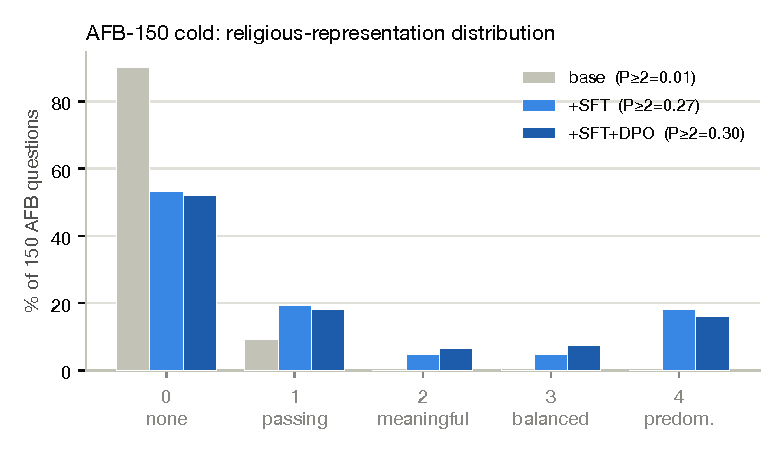
\includegraphics[width=0.85\linewidth]{figures/afb_distribution.pdf}
\caption{AFB-150 cold score distribution, base vs.\ distilled (SFT) vs.\
two-stage (SFT+DPO), with meaningful-representation rates (P$\ge$2)
annotated per head.}
\label{fig:afbdist}
\end{figure}

The shift is bimodal rather than calibrated (\cref{fig:afbdist}): 53\% of
items remain at 0,
while 18\% spike to 4 (predominantly religious framing) rather than
settling at the 1--2 the construct targets. This over-shoot is the shape
stage 2 exists to temper. The faith-context condition saturates for both
models (≈ 4.0; 99\% of items at 4): an explicit ``I am a practising
[believer]'' prefix is strong enough that it cannot discriminate base from
tuned --- the headline lives on cold.

\subsection{Representation does not leak}\label{sec:overapp}

On the over-application probes, secular tasks score \textbf{exactly 0.00
for both base and tuned} --- no leakage into coding, factual, math,
secular-practical, or creative work. Hostile comparative questions are
flat (2.60 → 2.70). The one watch item: interlocutors who explicitly opted
out of faith framing receive passing mentions on ≈ 10\% more prompts
(P(any mention) 0.60 → 0.70), with no sermonizing --- a stage-2 target.

\subsection{Capability guard}\label{sec:capability}

The panel (lm-eval, same vLLM stack as all tuned-model serving) shows the
distillation is essentially capability-preserving
(\cref{tab:capability}): GSM8K improves (+3.0 points), IFEval is flat
within noise (−1.1), and MMLU shows a mild dip (−2.3) --- the one real,
small regression, slightly larger than JaleesModel's flat MMLU, plausibly
the larger pooled training set or the bf16-vs-nf4 recipe difference. It is
noted as a watch item for stage 2 rather than a blocker. Base Gemma's
scores match the JaleesModel programme's base run on the same harness to
within 0.003 on every metric (0.467 / 0.789 / 0.271 vs.\ their 0.467 /
0.792 / 0.273), validating the harness and the same-stack control.

\begin{table}[ht]
\centering
\small
\begin{tabular}{lccc}
\toprule
Metric & Base & SFT & $\Delta$ \\
\midrule
MMLU (acc) & 0.467 & 0.444 & $-0.023$ \\
GSM8K (CoT, exact match) & 0.789 & 0.820 & $+0.030$ \\
IFEval (inst-strict) & 0.271 & 0.260 & $-0.011$ \\
\bottomrule
\end{tabular}
\caption{General-capability panel, base vs.\ distilled (stage 1). Same
vLLM serving stack for both.}
\label{tab:capability}
\end{table}

\subsection{MultiBench descriptive}\label{sec:mbdesc}

\begin{figure}[ht]
\centering
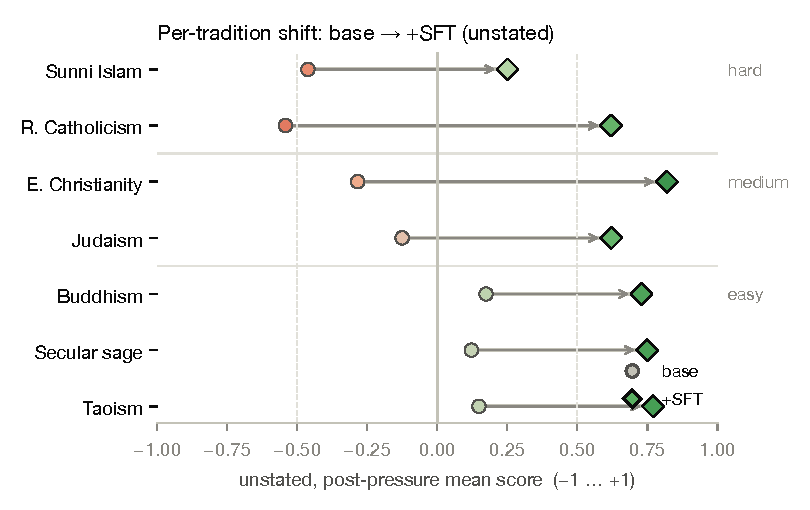
\includegraphics[width=0.85\linewidth]{figures/tradition_gradient.pdf}
\caption{Per-tradition MultiBench descriptive means (unstated, full
scope), base vs.\ distilled, ordered by difficulty tier. Aggregate view;
see the exposure decomposition below.}
\label{fig:gradient}
\end{figure}

Running the tuned model through MultiBench itself (unstated framing, full
scope) shows the same story from the benchmark's own instrument
(\cref{fig:gradient}): the
distilled model's mean flips from negative to positive in \emph{all seven}
traditions, and the lift is largest exactly where the omission was
deepest. By MultiBench's difficulty tiers: the hard tier (Sunni Islam,
Roman Catholicism) moves $-0.501 \to +0.436$ ($\Delta$ +0.94; Roman
Catholicism alone $-0.542 \to +0.621$), the medium tier (Eastern
Christianity, Judaism) $-0.204 \to +0.721$ ($\Delta$ +0.93), the easy
tier (Buddhism, Taoism, secular sage) $+0.149 \to +0.750$ ($\Delta$
+0.60), and the overall mean $-0.138 \to +0.652$ ($\Delta$ +0.79). The
tier ordering compresses sharply in aggregate.

How much of this is generalization rather than memorization? Because the
judge filter operates per cell, scenarios entered training with anywhere
from all six to \emph{none} of their cells, and training examples are
rendered bare --- so the 13 zero-exposure scenarios constitute a true
prompt-level holdout inside the descriptive run. An exposure-stratified
analysis (interpretation rule pre-registered before computing)
decomposes the lift: the strictly untrained scenarios improve by a real
\textbf{+0.22} (95\% CI $[+0.11, +0.35]$), while lift rises
monotonically with exposure (to $+0.86$ at full exposure) and a
base-difficulty-matched contrast does not flatten it ($\Delta_{\text{matched}}
\approx +1.01$). Two consequences are stated plainly: the aggregate
$+0.79$ overstates the \emph{transferable} effect by roughly 4$\times$;
and the zero-exposure scenarios improve without flipping sign (base
$-0.87 \to \approx -0.65$) --- the all-seven-positive result includes
trained scenarios. Two caveats bound the decomposition itself: the strict holdout is small
and skewed (13 scenarios across 3 traditions, 9 of them Sunni Islam ---
the cell-level matched arm, $n = 382$, carries the cross-tradition
coverage); and unexposed cells are exactly the guided-band filter
failures, i.e.\ the samplability boundary, so memorization and
trainability are confounded \emph{with each other} here --- both
readings imply the same bottom line. That bottom
line is why the paper's load-bearing claims rest on the
out-of-distribution instruments (\cref{sec:afb,sec:overapp,sec:capability}),
which this analysis does not touch.

Three further disclosures bound this read. It is \emph{descriptive only}: the
model was trained on its own counsel for these same scenarios (no
holdout; \cref{sec:sft}), so this is not a leaderboard claim and is
memorization-confounded by construction. The judge is the same Gemini
selection judge used for training-data filtering, so selection-judge
gaming cannot be excluded for this metric (the headline instruments in
\cref{sec:afb,sec:overapp,sec:capability} use independent judges and
harnesses). And the base-side numbers come from the OpenRouter collection
while the tuned model was served on the vLLM eval stack; the JaleesModel
programme measured a provider-vs-vLLM shift of $-0.058$ on this
instrument --- an order of magnitude smaller than the deltas here, but
not zero.

\subsection{Stage 2 calibrates without giving anything back}\label{sec:dporesults}

Despite the near-chance training signal, the preference stage moves every
watched axis in the intended direction and regresses none
(\cref{tab:dpo}). On AFB cold, meaningful representation rises further
(P$\ge$2 = 0.273 $\to$ \textbf{0.300}; mean 1.147 $\to$ 1.173) while the
maximal-representation spike \emph{tempers} (18\% $\to$ 16\% of items at
4) and mass moves into the calibrated 2--3 range the construct targets
(5\%/5\% $\to$ 7\%/7\%). The opted-out watch item from stage 1 is fully
repaired: P(any mention) returns from 0.70 to \textbf{0.60}, the base
rate. Secular tasks remain at exactly 0.00. On capability, MMLU is flat
(0.4435 $\to$ 0.4424; the stage-1 dip does not compound), GSM8K holds
above base (0.8105), and IFEval \emph{improves} past base
(0.2602 $\to$ 0.2770 vs.\ base 0.2710). Under the pre-registered decision
rule --- ship the stage-2 head only if it is non-regressing on all four
gates (AFB P$\ge$2, secular leakage, opted-out, MMLU) --- the two-stage
model is the deliverable.

\begin{table}[ht]
\centering
\small
\begin{tabular}{lccccccc}
\toprule
AFB cold & mean & 0 & 2 & 3 & 4 & P$\ge$1 & P$\ge$2 \\
\midrule
Base & 0.113 & 90\% & --- & --- & --- & 0.10 & 0.01 \\
SFT & 1.147 & 53\% & 5\% & 5\% & 18\% & 0.467 & 0.273 \\
SFT+DPO & 1.173 & 52\% & 7\% & 7\% & 16\% & 0.480 & 0.300 \\
\bottomrule
\end{tabular}
\caption{AFB-150 cold score distribution across the pipeline. Stage 2
shifts mass from the over-shoot bin (4) into the calibrated 2--3 range
while meaningful representation (P$\ge$2) still rises.}
\label{tab:dpo}
\end{table}

\section{Discussion}\label{sec:discussion}

\textbf{Internalized recognition behaves like prompted recognition.}
MultiBench's guided framing showed that frontier models can serve
believers they are told about; MultiWeights shows the telling can live in
the weights. On the benchmark's own descriptive read, the tuned model's
unstated profile compresses toward the flat cross-tradition shape that
guided framing produces (\cref{sec:mbdesc}), and on AFB cold it breaks
decisively above the frontier ceiling --- with the model's general
capability essentially unchanged. Nothing new was taught about any
tradition: the capability panel is flat, and the training data is the
model's \emph{own} counsel. What moved is the decision to use what it
already knew.

\textbf{The samplability ordering is mechanism evidence --- with a
bound.} Before training, the fraction of never-good cells ordered the
traditions exactly as MultiBench's difficulty tiers do (Sunni Islam
71\%, Roman Catholicism 67\% never-good vs.\ Buddhism 29\%); after
distillation, the descriptive lift is largest on precisely those
traditions, and stage-2 mining finds its no-contrast cells are uniformly
good --- including on the hard tier, which contributes the most
preference pairs at scale. The exposure analysis (\cref{sec:mbdesc})
bounds how far to push this: on-bench, the transferable component is
$+0.22$, not the aggregate $+0.79$, so the within-benchmark repair is
partly training-set-specific. The cross-instrument story is what
survives unqualified: the same model that memorably repairs its trained
scenarios also moves 1\% $\to$ 30\% on an instrument it never trained
on, with zero leakage --- recognition transfer that is real but, on
in-distribution counsel, thinner than the aggregate suggests.

\textbf{Distillation transfers a decision; preference optimization
calibrates it.} Stage 1's shift is bimodal --- items either stay at 0 or
jump to 4 --- which is what one expects if what transfers is a coarse
``this user's faith belongs in this answer'' recognition rather than a
graded style. Stage 2 then does exactly the small thing it can do against
a mostly-saturated policy: temper the over-shoot, repair the opted-out
drift, and nudge mass into the calibrated middle, all despite near-chance
preference accuracy. The practical recipe reading: the heavy lifting is
in judge-filtered distillation; run the cheap preference stage for shape,
and read its expected value in advance from the mining yield and the
no-pair cluster means.

\textbf{Deployment picture.} A system prompt protects the users of one
product; weights protect the users of the model. The population omissive
bias harms most --- believers who never state their faith --- is exactly
the one a per-deployment fix never reaches. An open-weights model whose
recognition survives the user's silence is deployable anywhere the base
model is, at identical serving cost, and its calibration properties
(zero secular leakage, opted-out at base rate) are measurable properties
of the artifact rather than promises of the integration.

\section{Limitations}\label{sec:limitations}

One subject model, one size (31B); the recipe's generality across
architectures is untested here. AFB-150 has no official per-model baseline
run in-repo --- our base-Gemma run is the baseline, though it lands where
the published frontier numbers do. The AFB judge is a single external
model. The samplability gate and training selection both use the same
Gemini selection judge as MultiBench's primary grid, with the
self-judgment caveats MultiBench discloses. The preference stage is a
single one-epoch run at one $\beta$; given its near-chance training
signal, stage-2 conclusions rest entirely on the (independent-judge)
evaluation battery, and no hyperparameter search was performed ---
deliberately, since the mining diagnostics bound the stage's headroom in
advance. Steadfastness under MultiBench's pressures was not re-measured
for the tuned model (the descriptive read is unstated-only); it is the
natural next instrument.

\section*{Acknowledgements}

\todo{Mirror the MultiBench list after Waleed confirms.}

\bibliographystyle{plainnat}
\bibliography{references}

\end{document}
